\documentclass[11pt]{article}
\usepackage{graphicx}
\usepackage{siunitx}
\usepackage{cleveref}
\usepackage{keyval,kvoptions,fancyvrb,float,ifthen,calc,ifplatform,pdftexcmds,etoolbox,lineno}
\usepackage[utf8]{inputenc}
\usepackage[danish]{babel}
\usepackage[left=25mm, right=25mm, top=25mm, bottom=25mm]{geometry}
\usepackage{amsthm}
\setlength\parindent{0pt}
\usepackage{dcolumn}
%\usepackage{minted}
\usepackage{setspace}
\usepackage{tabularx}
\usepackage{booktabs}
\usepackage{multirow}
\usepackage{caption}

\title{Dokumentation}

\begin{document}

\begin{titlepage}

\newcommand{\HRule}{\rule{\linewidth}{0.5mm}} % Defines a new command for the horizontal lines, change thickness here

\center % Center everything on the page
 
%----------------------------------------------------------------------------------
%	HEADING SECTIONS
%----------------------------------------------------------------------------------

\textsc{\LARGE Aarhus School of Engineering}\\[1.0cm] % Name of your university/college
\textsc{\Large 2.SEMESTERPROJEKT}\\[0.1cm]
\textsc{\large E2PRJ2}\\[0.3cm]
\textsc{\large gruppe 10}\\[0.3cm] % Minor heading such as course title

%----------------------------------------------------------------------------------
%	TITLE SECTION
%----------------------------------------------------------------------------------

\HRule \\[0.4cm]
{ \huge \bfseries Smart Morning System - SMS}\\[0.1cm] % Title of your document
\HRule \\[0.6cm]

%----------------------------------------------------------------------------------
%	DATE SECTION
%----------------------------------------------------------------------------------

{\large \today}\\[0.5cm] % Date, change the \today to a set date if you want to be precise
 
%----------------------------------------------------------------------------------
%	AUTHOR SECTION
%----------------------------------------------------------------------------------

\begin{minipage}[t]{0.4\textwidth}
\raggedright \large
\emph{Forfattere:}\\
\begin{tabular}[t]{@{}r@{ }l@{}}
	201511621 & \textbf{Christian Brandstrup Bondesen}\\
	201511621 & \textbf{Emil Celik}\\
	201408914 & \textbf{Marc Auphong Bui}\\
	2015xxxxx & \textbf{Rasmus Lund}\\
	201406253 & \textbf{Simon Egeberg}\\
  \end{tabular}
\end{minipage}
~
\begin{minipage}[t]{0.4\textwidth}
\raggedleft \large
\emph{Vejleder:} \\
\textbf{Kim Bjerge} % Supervisor's Name
\vfill
\end{minipage}\\[0.8cm]


%----------------------------------------------------------------------------------
%	LOGO SECTION
%----------------------------------------------------------------------------------
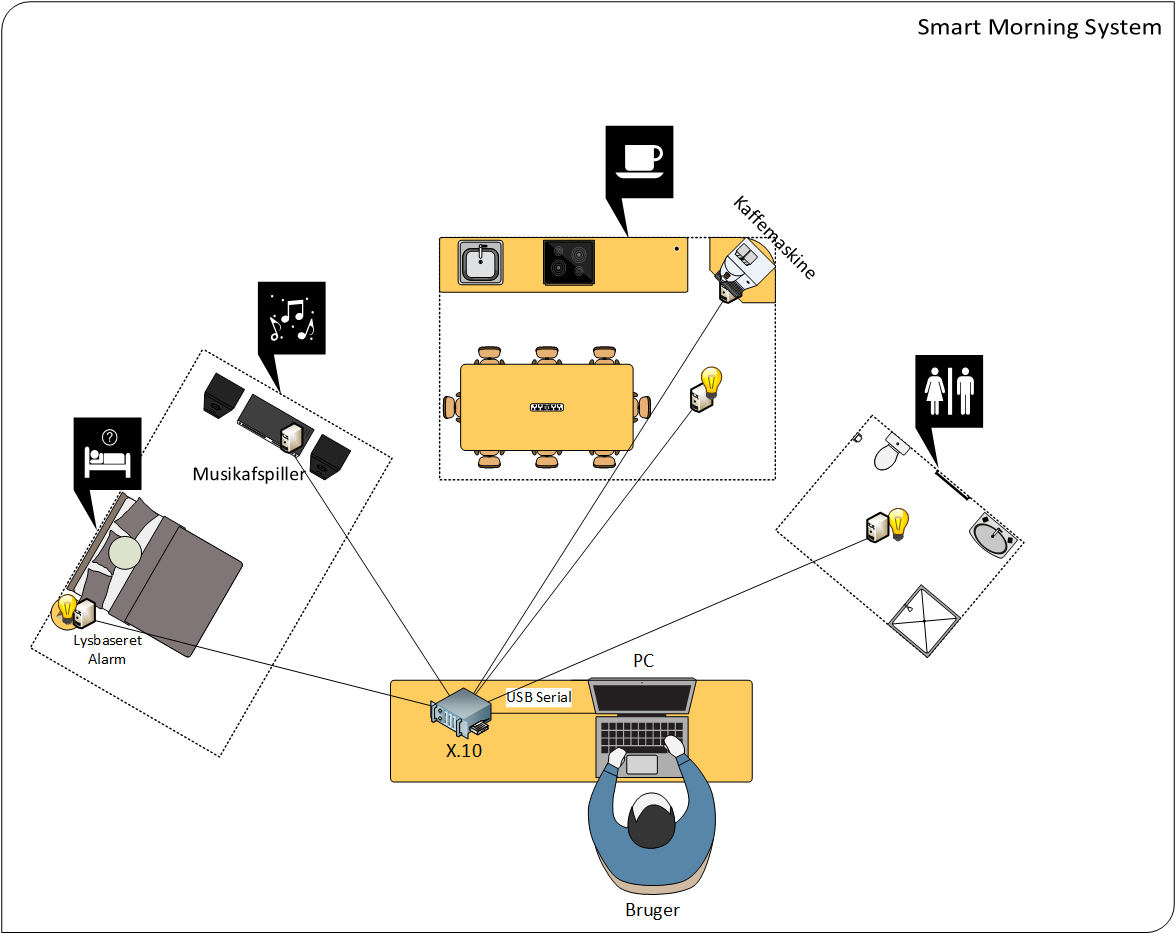
\includegraphics[scale=0.6]{projektillustration.png}\\[0.6cm]

\includegraphics[scale=0.25]{forsidelogo.jpg}\\[1cm] % Include a department/university logo - this will require the graphicx package
%----------------------------------------------------------------------------------
\vfill % Fill the rest of the page with whitespace

\end{titlepage}

\tableofcontents
\vfill
\pagebreak

\section{Indledning}
\vfill
\pagebreak

\section{Kravspecifikation}
%Tabeloversigt over hovedansvarsområder for projektdeltagerne
\vfill
\pagebreak

\section{Systemarkitektur}
%----------------------------------------------------------------------------------
%	Hardware-arkitektur
%----------------------------------------------------------------------------------
\subsection{Hardware-arkitektur}

%----------------------------------------------------------------------------------
%	Overordnet BDD
%----------------------------------------------------------------------------------
\subsubsection{BDD}

Det nedenstående block definition diagram (BDD) viser relationen mellem systemets elementer, og hvilke hovedelementer systemet består af.

\begin{figure}[H]
\centering
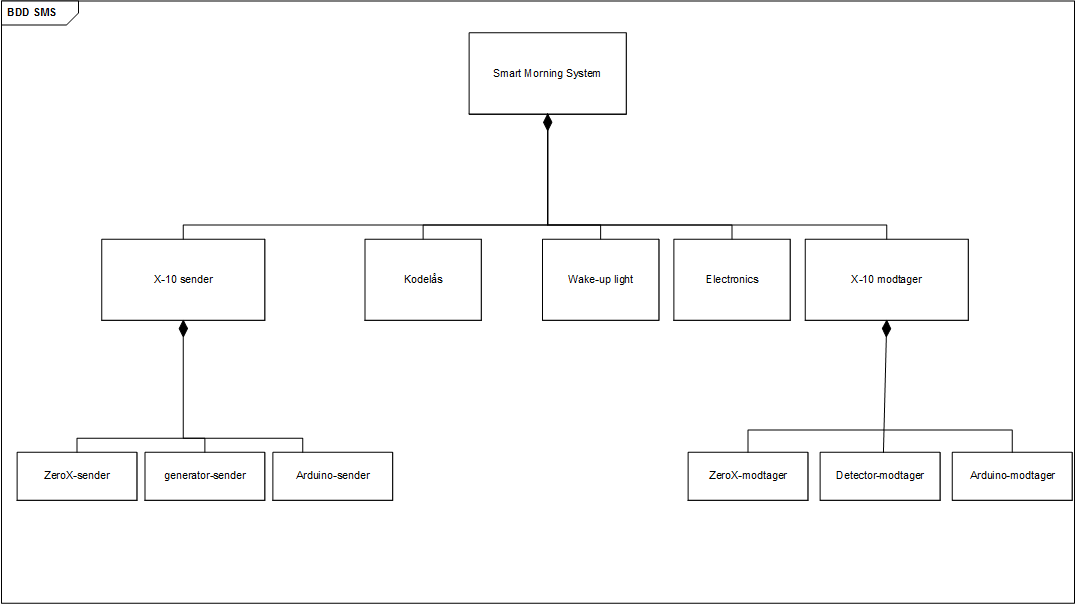
\includegraphics[width=\textwidth]{Bdd-sms-uden.png}
\caption{Overordnet BDD for Smart Morning System}
\label{fig: Overordnet_BDD_uden_ports}
\end{figure}

Som det ses illustreret i figur \ref{fig: Overordnet_BDD_uden_ports} består selve systemet i dets overordnet helhed af 5 moduler. X-10 Sender og X-10 Modtager står for at sende og modtage data over lysnettet ved brug af X-10 protokolen. Hvis X-10 Sender kan karakteriseres som hjernen, må X-10 Modtageren karakteriseres som de muskler der bevæger og fortæller hvordan legemer skal agere, altså hhv. Wake-up Light og Electronics.\pagebreak

En mere detaljeret BDD ses herunder, som også viser de enkelte blokkes ports.\newline

\begin{figure}[!ht]
	\centering
	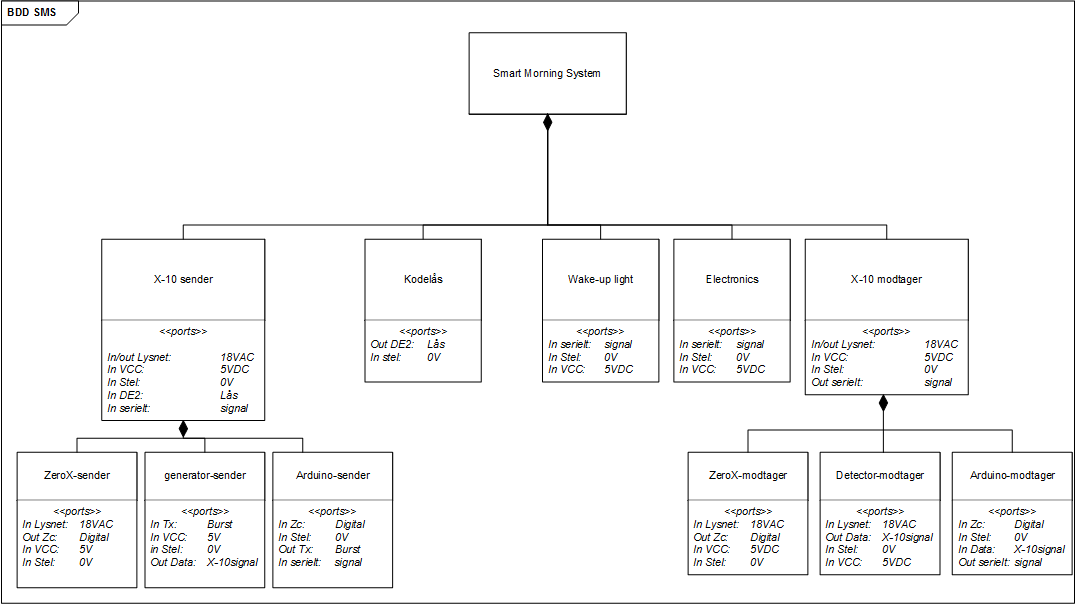
\includegraphics[width=\textwidth]{Bdd-sms.png}
	\caption{Detaljeret BDD for det overordnede Smart Morning System}
	\label{fig: Detaljeret BDD}
\end{figure}
\pagebreak


Den nedenstående tabel forklarer funktionen, de overordnede blokkes ansvar og signalnavne for de overordnede blokke.

\begin{table}[H]
\centering
	\begin{tabular}{l|p{10cm}|l|l}

	\toprule[0.4mm] \midrule
	\multicolumn{4}{c}{\textbf{Overordnet system}}\\
	\midrule[0.4mm] Bloknavn & Funktionsbeskrivelse & Signal & Kommentar\\ 
	\midrule[0.3mm]
	X-10 Sender & \multirow{2}{10cm}{Modtage data serielt fra PC og sende data over lysnettet, således det overlejret signal kan læses af X-10 Modtageren     \vfill} & 18V AC & Lysnet\\
	 & & 5V DC & VCC\\
	 & & 0V & Stel\\
	 & & Lås & DE2\\
	 & & Signal & Serielt\\
	 \midrule
	 Kodelås & \multirow{2}{10cm}{Sender højt eller lavt signal alt efter om systemet er låst eller ej  \vfill}& Lås & DE2\\
	 & & 0V & Stel\\
	 \midrule
	 Wake-up Light & \multirow{2}{10cm}{Tænder/slukker til et vis tidspunkt relativt til modtaget data fra X-10 modtageren \vfill}  & Signal & Serielt\\
	 & & 0V & Stel\\
	 & & 5V DC & VCC\\
	 \midrule
	 Electronics & \multirow{2}{10cm}{Tænder/slukker til et vis tidspunkt relativt til modtaget data fra X-10 modtageren \vfill}  & Signal & Serielt\\
	 & & 0V & Stel\\
	 & & 5V DC & VCC\\
	 \midrule
	 X-10 Modtager & \multirow{2}{10cm}{Modtage data fra lysnettet og sende videre til hhv. Modtager ATmega2560 og dernæst Wake-up Light og Electronics \vfill} & 18V AC & Lysnet\\
	 & & 5V DC & VCC\\
	 & & 0V & Stel\\
	 & & Signal & Serielt\\
	 \midrule\bottomrule[0.4mm]

	\end{tabular}
	\caption{Blokbeskrivelse for det overordnede system}
	\label{tab: Bloktabel}
\end{table}

%----------------------------------------------------------------------------------
%	Blokbeskrivelse X-10 Sender || ZeroX-sender
%----------------------------------------------------------------------------------

\subsubsection*{X-10 Sender Blokbeskrivelse}
Herunder vil de overstående blokke for X-10 Senderen nedbrydes yderligere, og de enkelte blokke vil blive forklaret.\newline

\begin{minipage}[Ht]{0.40\linewidth}
	\centering
	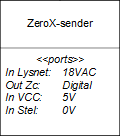
\includegraphics{ZeroX-sender-blok.png}
	%\captionof{figure}{ZeroX-sender Blok}\label{fig: ZeroX sender blok}
\end{minipage}
\hfill
\begin{minipage}[!t]{0.60\linewidth}
	\centering
  		 ZeroX-sender eller Zero Cross Detector på X-10 senderen, bruges til at detekere nulgennemgang og generere et firkant signal der kan tolkes logisk, hvor et højt signal betyder at der er nulgennemgang og omvendt. Dette bruges til at synkronisere hvornår der sendes og modtages data på lysnettet.
\end{minipage}%
\hfill

\begin{table}[H]
\centering
	\begin{tabular}{l|l|l}
	
	\toprule[0.4mm]\midrule \multicolumn{3}{c}{\textbf{ZeroX-sender Blok}}\\
	\midrule[0.4mm] Navn & Funktionsbeskrivelse & Signal\\ \midrule[0.3mm]
	 Lysnet & Modtage signal fra lysnettet & 18V AC\\
	 Zc & Sender digital signal til ATmega2560 & Digital\\
	 VCC & Spændingsforsyning til ZeroX-Detector & 5V DC\\
	 Stel & Fælles stel  & 0V\\
	 \midrule\bottomrule[0.4mm]

	\end{tabular}
	\caption{Blokbeskrivelse for senderens Zero Cross Detector}
	\label{tab: Bloktabel ZeroX sender}
\end{table}
\qquad

%----------------------------------------------------------------------------------
%	Blokbeskrivelse X-10 Sender || Generator-sender
%----------------------------------------------------------------------------------

\begin{minipage}[Ht]{0.40\linewidth}
	\centering
	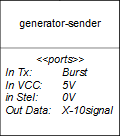
\includegraphics{Generator-sender-blok.png}
	%\captionof{figure}{Generator-sender Blok}\label{fig: Generator sender blok}
\end{minipage}
\hfill
\begin{minipage}[!t]{0.60\linewidth}
	\centering
   		Generator-sender eller 120kHz Carrier Generator bruges, i dette projekt, hovedsageligt til at sende data sikkert, altså de 120kHz, ud på lysnettet som er 50 Hz. 
\end{minipage}%
\hfill

\begin{table}[H]
\centering
	\begin{tabular}{l|l|l}
	
	\toprule[0.4mm]\midrule \multicolumn{3}{c}{\textbf{Generator-sender Blok}}\\
	\midrule[0.4mm] Navn & Funktionsbeskrivelse & Signal\\ \midrule[0.3mm]
	 Tx & Modtage Burstsignal fra sender ATmega2560 & Burst\\
	 VCC & Spændingsforsyning til Generatoren & 5V DC\\
	 Stel & Fælles stel  & 0V\\
 	 Data & Sender data signal til lysnettet & X-10 signal\\
	 \midrule\bottomrule[0.4mm]

	\end{tabular}
	\caption{Blokbeskrivelse for senderens Generator}
	\label{tab: Bloktabel Generator sender}
\end{table}
\qquad
%----------------------------------------------------------------------------------
%	Blokbeskrivelse X-10 Sender || Arduino-sender
%----------------------------------------------------------------------------------

\begin{minipage}[Ht]{0.40\linewidth}
	\centering
	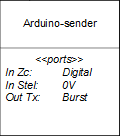
\includegraphics{Arduino-sender-blok.png}
	%\captionof{figure}{Arduino-sender Blok}\label{fig: Arduino sender blok}
\end{minipage}
\hfill
\begin{minipage}[!t]{0.60\linewidth}
	\centering
   		Arduino-sender eller ATmega2560 på senderen fungerer som en controlenhed og som det system der oversættet data fra pc og videre til 1 og 0'er til lysnettet, ved hver nulgennemgang. 
 \end{minipage}%
\hfill

\begin{table}[H]
\centering
	\begin{tabular}{l|l|l}
	
	\toprule[0.4mm]\midrule \multicolumn{3}{c}{\textbf{Arduino-sender Blok}}\\
	\midrule[0.4mm] Navn & Funktionsbeskrivelse & Signal\\ \midrule[0.3mm]
	 Zc & Modtage digitalt ZeroX signal fra ZeroX Detector & Digital\\
	 Stel & Fælles stel  & 0V\\
	 Tx & Sender 120kHz burst i perioder af 1 ms & Burst\\
	 \midrule\bottomrule[0.4mm]

	\end{tabular}
	\caption{Blokbeskrivelse for senderens ATmega2560}
	\label{tab: Bloktabel ATmega2560 sender}
\end{table}
\qquad

%----------------------------------------------------------------------------------
%	Blokbeskrivelse X-10 Modtager || ZeroX-modtager
%----------------------------------------------------------------------------------

\subsubsection*{X-10 Modtager Blokbeskrivelse}
Herunder vil de overstående blokke for X-10 Senderen nedbrydes yderligere, og de enkelte blokke vil blive forklaret.\newline

\begin{minipage}[Ht]{0.40\linewidth}
	\centering
	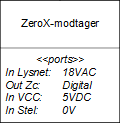
\includegraphics{ZeroX-modtager-blok.png}
	%\captionof{figure}{ZeroX-sender Blok}\label{fig: ZeroX sender blok}
\end{minipage}
\hfill
\begin{minipage}[!t]{0.60\linewidth}
	\centering
   		ZeroX-modtager eller Zero Cross Detector for X-10 Modtageren fungerer ligesom Zero Cross Detector i X-10 Senderen.
\end{minipage}%
\hfill

\begin{table}[H]
\centering
	\begin{tabular}{l|l|l}
	
	\toprule[0.4mm]\midrule \multicolumn{3}{c}{\textbf{ZeroX-modtager Blok}}\\
	\midrule[0.4mm] Navn & Funktionsbeskrivelse & Signal\\ \midrule[0.3mm]
	 Lysnet & Modtage signal fra lysnettet & 18V AC\\
	 Zc & Sender digital signal til ATmega2560 & Digital\\
	 VCC & Spændingsforsyning til ZeroX-Detector & 5V DC\\
	 Stel & Fælles stel  & 0V\\
	 \midrule\bottomrule[0.4mm]

	\end{tabular}
	\caption{Blokbeskrivelse for modtagerens Zero Cross Detector}
	\label{tab: Bloktabel ZeroX modtager}
\end{table}
\qquad
%----------------------------------------------------------------------------------
%	Blokbeskrivelse X-10 Modtager || Detector-modtager
%----------------------------------------------------------------------------------

\begin{minipage}[Ht]{0.40\linewidth}
	\centering
	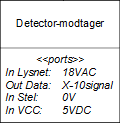
\includegraphics{Detector-modtager-blok.png}
	%\captionof{figure}{Generator-sender Blok}\label{fig: Generator sender blok}
\end{minipage}
\hfill
\begin{minipage}[!t]{0.60\linewidth}
	\centering
   		Detector-modtager eller \SI{120}{\kilo \Hz} Carrier Detector er den blok der skal stå for at modtage det overlejrede signal fra lysnettet, og filtrere de \SI{120}{\kilo \Hz} fra de \SI{50}{\Hz}, og konvertere det signal om til et data signal der kan læses af ATmega2560 på X-10 Modtageren.
\end{minipage}%
\hfill

\begin{table}[H]
\centering
	\begin{tabular}{l|l|l}
	
	\toprule[0.4mm]\midrule \multicolumn{3}{c}{\textbf{Detector-modtager Blok}}\\
	\midrule[0.4mm] Navn & Funktionsbeskrivelse & Signal\\ \midrule[0.3mm]
	 Lysnet & Modtage overlejret signal fra lysnettet & 18V AC\\
	 Data & Sender data signal til ATmega2560 & X-10 signal\\
	 Stel & Fælles stel  & 0V\\
	 VCC & Spændingsforsyning til Generatoren & 5V DC\\
 	 
	 \midrule\bottomrule[0.4mm]

	\end{tabular}
	\caption{Blokbeskrivelse for modtagerens Detector}
	\label{tab: Bloktabel Detector modtager}
\end{table}
\qquad
%----------------------------------------------------------------------------------
%	Blokbeskrivelse X-10 Modtager || Arduino-modtager
%----------------------------------------------------------------------------------

\begin{minipage}[Ht]{0.40\linewidth}
	\centering
	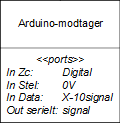
\includegraphics{Arduino-modtager-blok.png}
	%\captionof{figure}{Arduino-sender Blok}\label{fig: Arduino sender blok}
\end{minipage}
\hfill
\begin{minipage}[!t]{0.60\linewidth}
	\centering
   		Arduino-modtager elloer ATmega2560 på X-10 modtageren, modtager data signalet fra 120 kHz Carrier Detector, og oversætter dette signal til hhv. Wake-up Light og Electronics. Ligeledes bruges Zero Cross Detectoren til at synkronisere hvornår der skal læses data.
\end{minipage}%
\hfill

\begin{table}[H]
\centering
	\begin{tabular}{l|l|l}
	
	\toprule[0.4mm]\midrule \multicolumn{3}{c}{\textbf{Arduino-modtager Blok}}\\
	\midrule[0.4mm] Navn & Funktionsbeskrivelse & Signal\\ \midrule[0.3mm]
	 Zc & Modtage digitalt ZeroX signal fra ZeroX Detector & Digital\\
	 Stel & Fælles stel  & 0V\\
	 Data & Modtage data signal fra Detektor & X-10 signal\\
	 Serielt & Sender signal til Wake-up Light og Electronics med X-10 data & Signal\\
	 \midrule\bottomrule[0.4mm]

	\end{tabular}
	\caption{Blokbeskrivelse for modtagerens Arduino}
	\label{tab: Bloktabel_Arduino_modtager}
\end{table}
\qquad


\pagebreak
%----------------------------------------------------------------------------------
%	IBD - Hardware Systemarkitektur
%----------------------------------------------------------------------------------
\subsubsection{IBD}

For at forklare sammenhængen og forbindelsen mellem de enkelte HW-blokke, illustreres de ved internal block diagrams (IBD) for hhv. X-10 Sender og X-10 Modtager.\\

Herunder ses IBD'en for X-10 Senderen. Signalerne er yderligere beskrevet i signalbeskrivelsestabellerne længere nede. 

\begin{figure}[!ht]
	\centering
	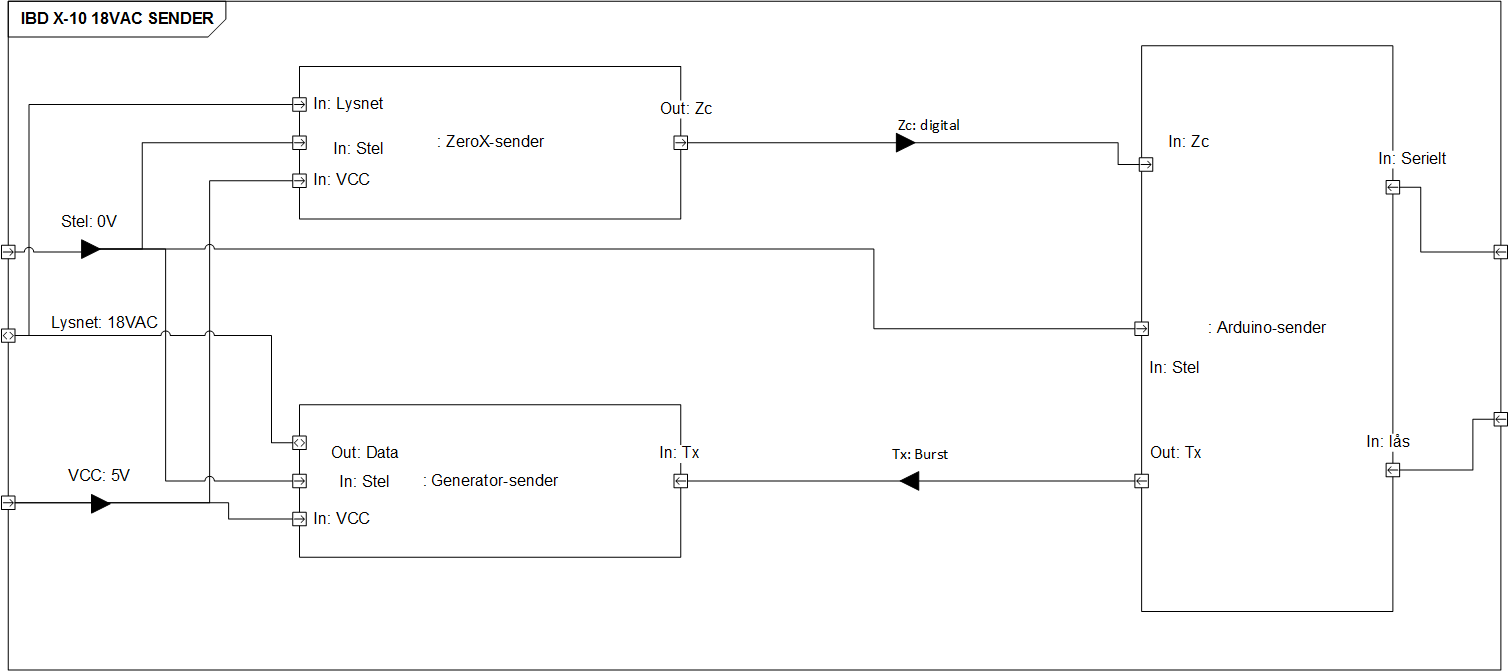
\includegraphics[width=\textwidth]{IBD_sender.png}
	\caption{IBD for X-10 Senderen}
	\label{fig: IBD X-10 Sender}
\end{figure}

Herunder ses IBD'en for X-10 Modtageren. Signalerne er yderligere beskrevet i signalbeskrivelsestabellerne længere nede. 

\begin{figure}[!ht]
	\centering
	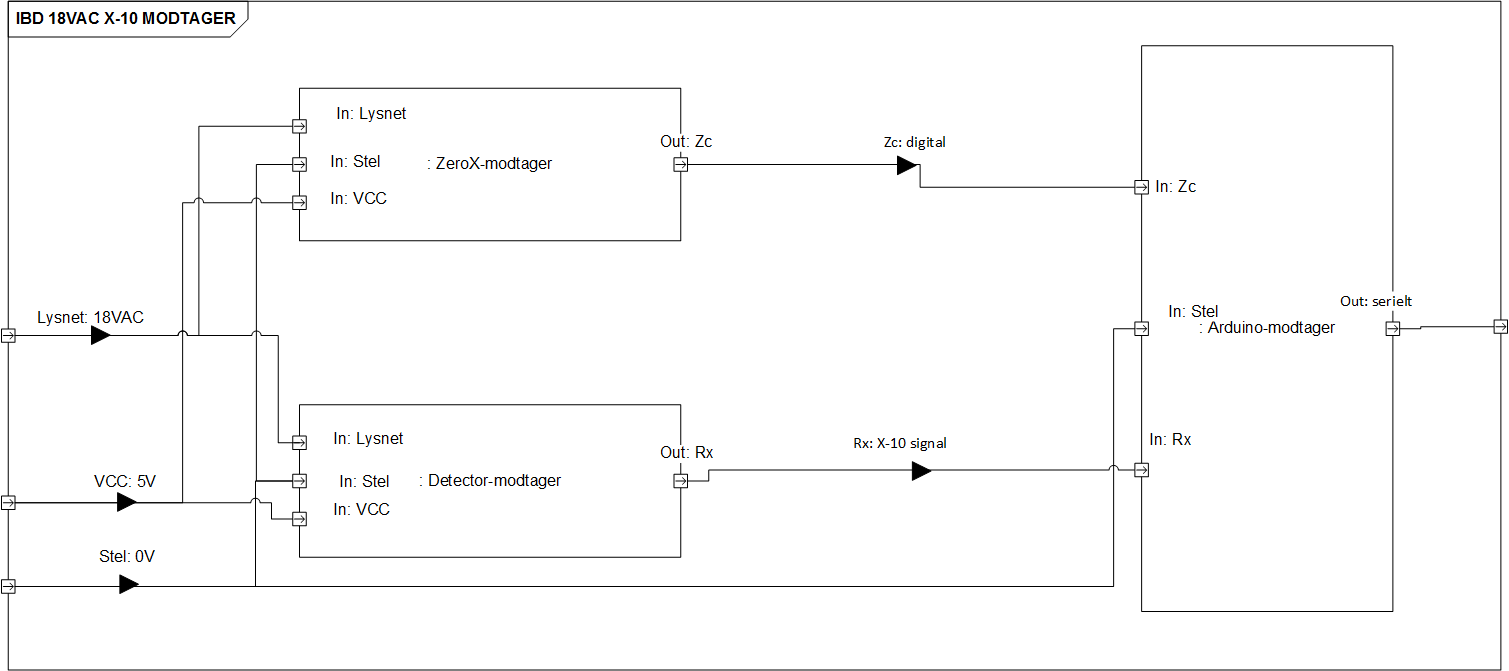
\includegraphics[width=\textwidth]{IBD_modtager.png}
	\caption{IBD for X-10 Modtageren}
	\label{fig: IBD X-10 Modtager}
\end{figure}

\subsubsection*{Signalbeskrivelse}
I nedenstående tabel beskrives signalerne i forbindelserne vist i hhv. figur \ref{fig: IBD X-10 Sender} og fig \ref{fig: IBD X-10 Modtager}.

\begin{table}[H]
\centering
	\begin{tabularx}{\textwidth}{X|p{4cm}|X|p{2.9cm}|p{2.9cm}|X}

	\toprule[0.4mm] \midrule \multicolumn{6}{c}{\textbf{Signalbeskrivelse}}\\
	\midrule \toprule[0.4mm] \multicolumn{6}{c}{\textbf{X-10 Sender}}\\
	\midrule[0.4mm] Signal & Funktionsbeskrivelse & Område & Port In & Port Out & Kom.\\ 
	\midrule[0.3mm]
	18VAC & Signal fra lysnettet & 18VAC & ZeroX: Lysnet & Lysnettet &\\
	& & & Lysnettet & Generator: Data &\\
	\midrule
	5V & Forsyningsspænding & 5V DC & ZeroX: VCC & Forsyning &\\
	&  &  & Generator: VCC & Forsyning &\\
	\midrule
	0V & Stel/Reference & 0V & ZeroX: Stel & Reference &\\
	&  &  & Generator: Stel & Reference &\\
	&  &  & Arduino: Stel & Reference &\\
	\midrule
	digital & Digitalt Zero Cross signal & 0.2-5 V & Arduino: Zc & ZeroX: Zc &\\
	\midrule
	Burst & \SI{120}{\kilo \Hz} burst fra ATmega2560 & \SI{120}{\kilo \Hz} & Generator: Tx & Arduino: Tx &\\
	\midrule
	Serielt & Seriel data fra PC &  & Arduino: Serielt & PC &\\
	\midrule
	lås & Logisk låse signal & 0.2-5 V & Arduino: lås & Kodelås &\\
	%X-10 Modtager -->
	\midrule[0.4mm] \multicolumn{6}{c}{\textbf{X-10 Modtager}}\\
	\midrule[0.4mm] Signal & Funktionsbeskrivelse & Område & Port In & Port Out & Kom.\\ \midrule[0.3mm]
	18VAC & Signal fra lysnettet & 18VAC & ZeroX: Lysnet & Lysnettet &\\
	& & & Lysnettet & Detector: Lysnet &\\
	\midrule
	5V & Forsyningsspænding & 5V DC & ZeroX: VCC & Forsyning &\\
	&  &  & Detector: VCC & Forsyning &\\
	\midrule
	0V & Stel/Reference & 0V & ZeroX: Stel & Reference &\\
	&  &  & Detector: Stel & Reference &\\
	&  &  & Arduino: Stel & Reference &\\
	\midrule
	digital & Digitalt Zero Cross signal & 0.2-5 V & Arduino: Zc & ZeroX: Zc &\\
	\midrule
	X-10 signal & \SI{120}{\kilo \Hz} burst fra ATmega2560 & \SI{120}{\kilo \Hz} & Generator: Tx & Arduino: Tx &\\
	\midrule
	serielt & Seriel data fra lysnettet oversat af protokol &  & Arduino: serielt & Wake-up Light, Electronics &\\
	\midrule\bottomrule[0.4mm]


	\end{tabularx}
	\caption{Signalbeskrivelse for både X-10 Sender og Modtager}
	\label{tab: signalbeskrivelse}
\end{table}




%----------------------------------------------------------------------------------
%	Software-arkitektur
%----------------------------------------------------------------------------------
\subsection{Software-arkitektur}

\vfill
\pagebreak

\section{Hardware-design, implementering \& modultest}
\subsection{Design (HW)}
\subsection{Implementering (HW)}
\subsection{Modultest (HW)}
\vfill
\pagebreak

\section{Software-design, implementering \& modultest}
\subsection{Design (SW)}
\subsection{Implementering (SW)}
\subsection{Modultest (SW)}
\vfill
\pagebreak

\section{Integrationstest (HW/SW)}
%Valgfrit på 2.semester
\vfill
\pagebreak

\section{Accepttest}
\vfill
\pagebreak

\section{Bilag}
\vfill
\pagebreak



\end{document}
